\documentclass[german,a5paper, twoside]{scrreprt} %report veraltet, scrreprt neu
%Packages
\usepackage{geometry} %Definition Satzspiegel
\geometry{left=2cm,right=2cm,top=2.1cm,bottom=2.2cm} 
\usepackage[ngerman]{babel}%auch für Umlaute???
\usepackage{bibgerm}%deutsche trennung
\usepackage[utf8]{inputenc}%Zeichensatz
\usepackage[T1]{fontenc}%fontsatz
\usepackage{geometry}
\geometry{a5paper}
\usepackage{setspace} 
\usepackage{musixtex} 
\usepackage{musixguit}
\usepackage{graphicx} %Graphiken
\usepackage{float}
\usepackage{placeins}
\usepackage{pdfpages}%mehrseitige PDFs einbinden
\usepackage{fancyhdr}%Kopfzeilen usw.


%\makeindex[name=titel, title=Inhalt,options=-s mkidx]
%\makeindex[name=anfang, title=Inhalt,options=-s mkidx]
%options=-s index_glossar_und_
%abkuerzungsverzeichnis-bsp02]
%\makeindex[%
%name=autor,%
%title=Autorenverzeichnis,%
%intoc,
%options=-s index_glossar_und_
%abkuerzungsverzeichnis-bsp02%

%\indexsetup{%
%level=\subsection*,%
%toclevel=subsection,%
%noclearpage%
%}
%\makeatletter
%\newcommand{\imki@idxprologue}{}
%\makeatother




\makeatletter%Zeilenabstand anpassen Inhaltsverzeichnis
%\renewcommand{\l@chapter}{\@dottedtocline{2}{0.8em }{0.8em}}
\renewcommand{\l@subsection}{\@dottedtocline{2}{1.5em}{3.3em}}
\makeatother


\newcommand{\chort}[2]{\chord{\textbf{#1}}{#2}}
\usepackage{hyperref}

\begin{document}

\begin{figure}[H]
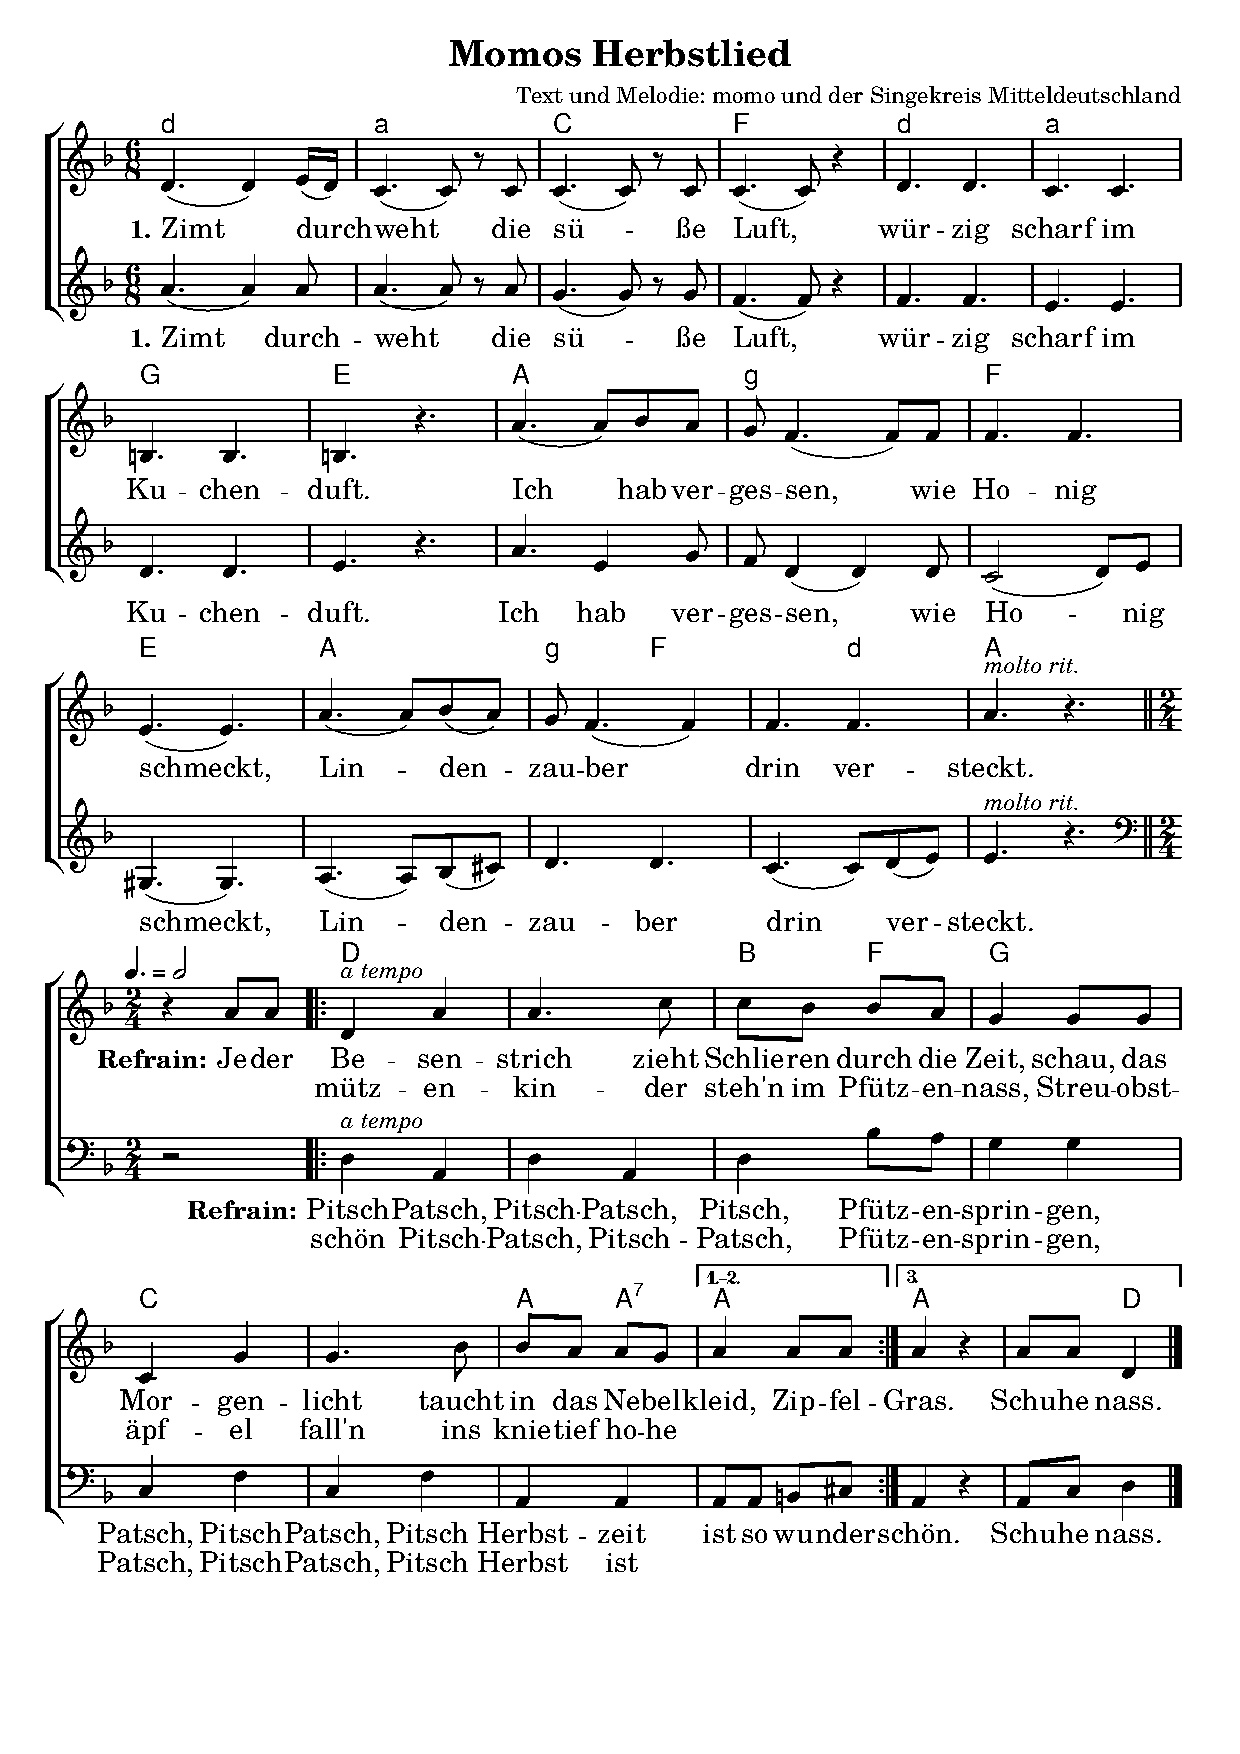
\includepdf[trim=00mm 5mm 00mm 00mm,pagecommand={},pages=1,width=1.3\textwidth]{Rohdaten/Noten/Herbstlied_Noten.pdf}
\end{figure}
\vspace{20cm}
\begin{song} \noindent


\textbf{2.}

\chort{d}{Heißer} \chort{a}{Tee} und \chort{C}{Funken}\chort{F}{glut}
\chort{d}{Spühlen} \chort{a}{Hitze} \chort{G}{in} das \chort{E}{Blut.}
\chort{A}{Deine} \chort{g}{Hände} \chort{F}{warm} und \chort{E}{weich}
\chort{A}{streifen} \chort{g}{Meine} \chort{F}{windhauch}\chort{A}{gleich.}

\textbf{Refrain:} 

Jeder \chort{D}{Besenstrich} zieht \chort{B}{Schlieren} \chort{F}{durch} die \chort{G}{Zeit}
Schau das \chort{C}{Morgenlicht} taucht \chort{A}{in} das \chort{A$^7$}{Nebel}\chort{A}{kleid}
Zipfel\chort{D}{mützenkinder} \chort{B}{steh’n} im \chort{F}{Pfützen}\chort{G}{nass}
Streuobst\chort{C}{äpfel} fall’n ins \chort{A}{knietief} \chort{A$^7$}{hohe} \chort{A}{Gras}

\textbf{3.}
\chort{d}{Zärtlich} \chort{a}{klingt} ein \chort{C}{kleines} \chort{F}{Lied}
\chort{d}{spricht} da\chort{a}{von} \chort{G}{wie} Glück ge\chort{E}{schieht.}
\chort{A}{kleine} \chort{g}{Töne,} \chort{F}{leises} \chort{E}{Wort,}
\chort{A}{finden} \chort{g}{Ohren} an \chort{F}{ihrem}\chort{A}{Ort.}\\[0.5em]
\end{song}


\end{document}
